% ===== logistic-regression =====
\section*{Logistic Regression}

\subsection*{What Logistic Regression Does}
Logistic regression is similar to linear regression, except it predicts the \textbf{probability} that something is true (a number between 0 and 1) rather than an unbounded real-valued quantity.

\begin{itemize}
  \item Example: input $\mathbf{x}$ = measurements of a tumor, output = probability it's cancer.
  \item This is \textbf{supervised classification}: we get labeled pairs $(\mathbf{x}, t)$ with $t \in \{0, 1\}$. It's \textbf{discriminative}: it models $P(C_1 \mid \mathbf{x})$ directly.
\end{itemize}

\subsection*{The Sigmoid}
\begin{keeptogether}
The sigmoid turns any number into a probability:
\[
\sigma(a) = \frac{1}{1 + e^{-a}}
\qquad \text{e.g.}\quad
\sigma(-3) = 0.05, \quad \sigma(0) = 0.5, \quad \sigma(3) = 0.95
\]

{\centering
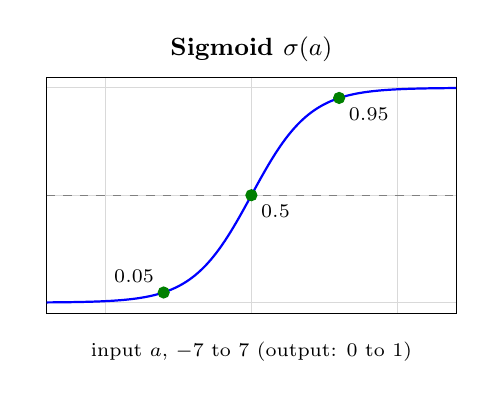
\begin{tikzpicture}
\begin{axis}[scale only axis, width=5.2cm, height=3cm,
    xmin=-7, xmax=7, ymin=-0.05, ymax=1.05, enlargelimits=false,
    grid=major, grid style={gray!30}, major tick length=0pt,
    xticklabels={}, yticklabels={},
    title={\small\textbf{Sigmoid $\sigma(a)$}}, title style={yshift=-4pt},
    xlabel={\scriptsize input $a$, $-7$ to $7$ (output: 0 to 1)}, label style={font=\scriptsize}]
\addplot[gray, dashed] coordinates {(-7,0.5) (7,0.5)};
\addplot[thick, blue, domain=-7:7, samples=150] {1/(1+exp(-x))};
\addplot[only marks, mark=*, green!50!black, mark size=2pt] coordinates {(-3,0.047) (0,0.5) (3,0.953)};
\node[font=\scriptsize, anchor=south east] at (axis cs:-3,0.047) {$0.05$};
\node[font=\scriptsize, anchor=north west] at (axis cs:0,0.5) {$0.5$};
\node[font=\scriptsize, anchor=north west] at (axis cs:3,0.953) {$0.95$};
\end{axis}
\end{tikzpicture}
\par}
\end{keeptogether}

\begin{itemize}
  \item Big negative input $\to$ near 0. Big positive input $\to$ near 1. Input $0 \to$ exactly $0.5$.
  \item \textbf{Big idea:} logistic regression = linear regression's output $\mathbf{w}^\top\mathbf{x}$ passed through $\sigma$.
\end{itemize}

\subsection*{Running Example: Tumor Radius}
Predict whether a tumor is \textbf{cancer} ($t = 1$, class $C_1$) or \textbf{not cancer} ($t = 0$, class $C_2$) from one feature: its radius $x$.

\begin{keeptogether}
{\centering
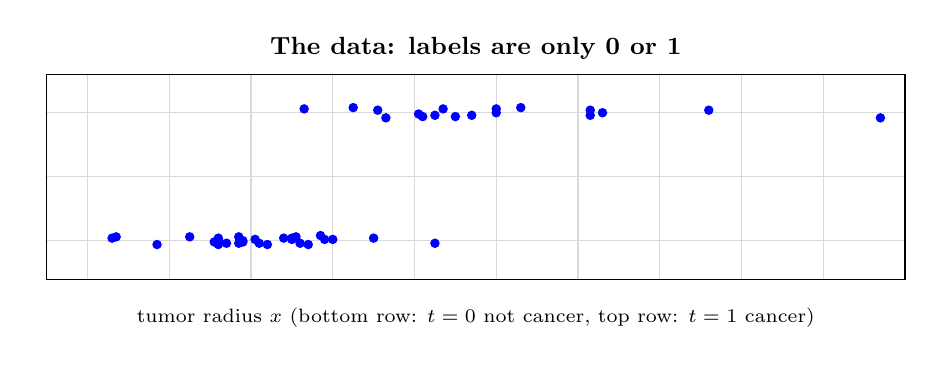
\begin{tikzpicture}
\begin{axis}[scale only axis, width=10.9cm, height=2.6cm,
    xmin=7, xmax=28, ymin=-0.3, ymax=1.3, enlargelimits=false,
    grid=major, grid style={gray!30}, major tick length=0pt,
    xticklabels={}, yticklabels={},
    title={\small\textbf{The data: labels are only 0 or 1}}, title style={yshift=-4pt},
    xlabel={\scriptsize tumor radius $x$ (bottom row: $t = 0$ not cancer, top row: $t = 1$ cancer)}, label style={font=\scriptsize}]
\addplot[only marks, mark=*, blue, mark size=1.5pt] coordinates {
  (8.6,0.02) (8.7,0.03) (9.7,-0.03) (10.5,0.03) (11.1,-0.01) (11.2,-0.00) (11.2,-0.03) (11.2,0.02)
  (11.4,-0.02) (11.7,0.03) (11.7,-0.02) (11.8,0.00) (11.8,-0.01) (12.1,0.01) (12.2,-0.02) (12.4,-0.03)
  (12.8,0.02) (13.0,0.02) (13.0,0.01) (13.1,0.03) (13.2,-0.02) (13.3,1.03) (13.4,-0.03) (13.7,0.04)
  (13.8,0.01) (14.0,0.01) (14.5,1.04) (15.0,0.02) (15.1,1.02) (15.3,0.96) (16.1,0.99) (16.2,0.97)
  (16.5,-0.02) (16.5,0.98) (16.7,1.03) (17.0,0.97) (17.4,0.98) (18.0,1.00) (18.0,1.03) (18.6,1.04)
  (20.3,1.02) (20.3,0.98) (20.6,1.00) (23.2,1.02) (27.4,0.96)};
\end{axis}
\end{tikzpicture}
\par}
\end{keeptogether}

\begin{itemize}
  \item Small tumors are mostly not cancer and large ones mostly cancer, with some overlap in the middle.
  \item We want a curve that gives $P(\text{cancer} \mid x)$ for every radius.
\end{itemize}

\subsection*{Why Not a Straight Line?}
\begin{keeptogether}
Fit least squares to the 0/1 labels and the line keeps going: it predicts $-0.34$ at radius 7 and $1.76$ at radius 28. Those aren't probabilities. The sigmoid flattens out at 0 and 1 instead.

{\centering
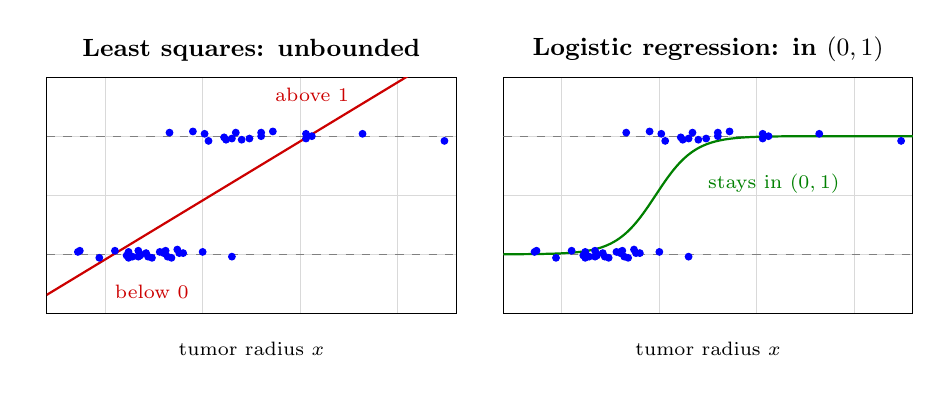
\begin{tikzpicture}
% ---- least squares ----
\begin{axis}[name=lin, scale only axis, width=5.2cm, height=3cm,
    xmin=7, xmax=28, ymin=-0.5, ymax=1.5, enlargelimits=false, clip=true,
    grid=major, grid style={gray!30}, major tick length=0pt,
    xticklabels={}, yticklabels={},
    title={\small\textbf{Least squares: unbounded}}, title style={yshift=-4pt},
    xlabel={\scriptsize tumor radius $x$}, label style={font=\scriptsize}]
\addplot[gray, dashed] coordinates {(7,0) (28,0)};
\addplot[gray, dashed] coordinates {(7,1) (28,1)};
\addplot[only marks, mark=*, blue, mark size=1.2pt] coordinates {
  (8.6,0.02) (8.7,0.03) (9.7,-0.03) (10.5,0.03) (11.1,-0.01) (11.2,-0.00) (11.2,-0.03) (11.2,0.02)
  (11.4,-0.02) (11.7,0.03) (11.7,-0.02) (11.8,0.00) (11.8,-0.01) (12.1,0.01) (12.2,-0.02) (12.4,-0.03)
  (12.8,0.02) (13.0,0.02) (13.0,0.01) (13.1,0.03) (13.2,-0.02) (13.3,1.03) (13.4,-0.03) (13.7,0.04)
  (13.8,0.01) (14.0,0.01) (14.5,1.04) (15.0,0.02) (15.1,1.02) (15.3,0.96) (16.1,0.99) (16.2,0.97)
  (16.5,-0.02) (16.5,0.98) (16.7,1.03) (17.0,0.97) (17.4,0.98) (18.0,1.00) (18.0,1.03) (18.6,1.04)
  (20.3,1.02) (20.3,0.98) (20.6,1.00) (23.2,1.02) (27.4,0.96)};
\addplot[thick, red!80!black, domain=7:28, samples=2] {0.100*x - 1.044};
\node[font=\scriptsize, red!80!black, anchor=west] at (axis cs:10,-0.32) {below 0};
\node[font=\scriptsize, red!80!black, anchor=east] at (axis cs:23,1.35) {above 1};
\end{axis}
% ---- logistic regression ----
\begin{axis}[name=log, at={(lin.east)}, anchor=west, xshift=0.6cm,
    scale only axis, width=5.2cm, height=3cm,
    xmin=7, xmax=28, ymin=-0.5, ymax=1.5, enlargelimits=false,
    grid=major, grid style={gray!30}, major tick length=0pt,
    xticklabels={}, yticklabels={},
    title={\small\textbf{Logistic regression: in $(0,1)$}}, title style={yshift=-4pt},
    xlabel={\scriptsize tumor radius $x$}, label style={font=\scriptsize}]
\addplot[gray, dashed] coordinates {(7,0) (28,0)};
\addplot[gray, dashed] coordinates {(7,1) (28,1)};
\addplot[only marks, mark=*, blue, mark size=1.2pt] coordinates {
  (8.6,0.02) (8.7,0.03) (9.7,-0.03) (10.5,0.03) (11.1,-0.01) (11.2,-0.00) (11.2,-0.03) (11.2,0.02)
  (11.4,-0.02) (11.7,0.03) (11.7,-0.02) (11.8,0.00) (11.8,-0.01) (12.1,0.01) (12.2,-0.02) (12.4,-0.03)
  (12.8,0.02) (13.0,0.02) (13.0,0.01) (13.1,0.03) (13.2,-0.02) (13.3,1.03) (13.4,-0.03) (13.7,0.04)
  (13.8,0.01) (14.0,0.01) (14.5,1.04) (15.0,0.02) (15.1,1.02) (15.3,0.96) (16.1,0.99) (16.2,0.97)
  (16.5,-0.02) (16.5,0.98) (16.7,1.03) (17.0,0.97) (17.4,0.98) (18.0,1.00) (18.0,1.03) (18.6,1.04)
  (20.3,1.02) (20.3,0.98) (20.6,1.00) (23.2,1.02) (27.4,0.96)};
\addplot[thick, green!50!black, domain=7:28, samples=150] {1/(1+exp(-(x-14.81)))};
\node[font=\scriptsize, green!50!black, anchor=west] at (axis cs:17,0.6) {stays in $(0,1)$};
\end{axis}
\end{tikzpicture}
\par}
\end{keeptogether}

\subsection*{Building the Model with Gradient Descent}
Same as gradient descent for linear regression: start at $\mathbf{w} = \mathbf{0}$ and take small downhill steps until the error stops going down. Only the model and the error change.

\begin{keeptogether}
\textbf{Step 1: What the weights control.} The model is always an S-curve, $y(\mathbf{x}, \mathbf{w}) = \sigma(w_0 + w_1 x) = \sigma(\mathbf{w}^\top\mathbf{x})$ with dummy feature $x_0 = 1$. The weights only move and stretch it: the center is at $x = -w_0/w_1$, and a bigger $w_1$ makes it steeper. Training picks the $(w_0, w_1)$ that fits best.

{\centering
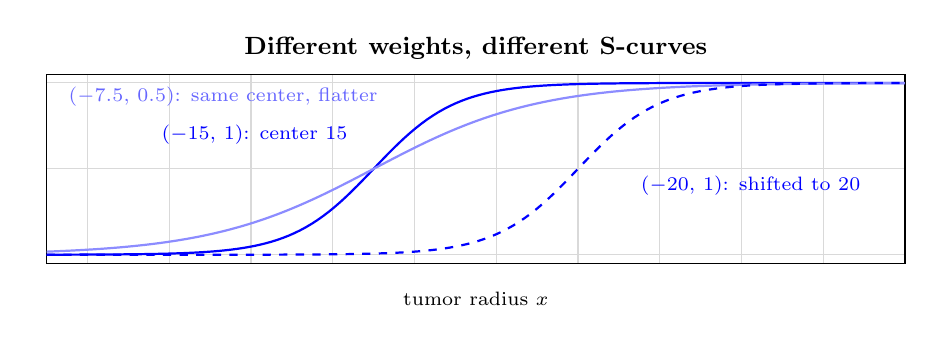
\begin{tikzpicture}
\begin{axis}[scale only axis, width=10.9cm, height=2.4cm,
    xmin=7, xmax=28, ymin=-0.05, ymax=1.05, enlargelimits=false,
    grid=major, grid style={gray!30}, major tick length=0pt,
    xticklabels={}, yticklabels={},
    title={\small\textbf{Different weights, different S-curves}}, title style={yshift=-4pt},
    xlabel={\scriptsize tumor radius $x$}, label style={font=\scriptsize}]
\addplot[thick, blue, domain=7:28, samples=150] {1/(1+exp(-(-15+x)))};
\addplot[thick, blue!45, domain=7:28, samples=150] {1/(1+exp(-(-7.5+0.5*x)))};
\addplot[thick, blue, dashed, domain=7:28, samples=150] {1/(1+exp(-(-20+x)))};
\node[font=\scriptsize, blue!60, anchor=west] at (axis cs:7.3,0.92) {$(-7.5,\,0.5)$: same center, flatter};
\node[font=\scriptsize, blue, anchor=east] at (axis cs:14.6,0.7) {$(-15,\,1)$: center 15};
\node[font=\scriptsize, blue, anchor=west] at (axis cs:21.3,0.4) {$(-20,\,1)$: shifted to 20};
\end{axis}
\end{tikzpicture}
\par}
\end{keeptogether}

\textbf{Step 2: Measure how bad a curve is.} Each tumor's error is $-\ln$ of the probability the curve gives its true label. For a tumor with cancer ($t = 1$), $y = 0.9$ costs $-\ln 0.9 = 0.11$ and $y = 0.1$ costs $-\ln 0.1 = 2.30$. Summing gives the \textbf{cross-entropy error}:
\[
E(\mathbf{w}) = -\sum_{n=1}^{N} \Big[\, \underbrace{t_n \ln y_n}_{\text{on if } t_n = 1} + \underbrace{(1 - t_n)\ln(1 - y_n)}_{\text{on if } t_n = 0} \,\Big],
\qquad y_n = \sigma(\mathbf{w}^\top\mathbf{x}_n)
\]
Why not squared distance $(y - t)^2$ like linear regression? It caps at 1, so a confidently wrong curve barely gets punished, and with the sigmoid it isn't convex (cross-entropy is).

\begin{keeptogether}
\textbf{Step 3: Take downhill steps.} To go downhill we need the derivative of $E$. For one tumor, chain rule through $y = \sigma(a)$ and $a = \mathbf{w}^\top\mathbf{x}$:
\[
\frac{\partial E}{\partial w_d}
= \underbrace{\Big(-\frac{t}{y} + \frac{1-t}{1-y}\Big)}_{\partial E / \partial y}
\cdot \underbrace{y(1-y)}_{\sigma'(a)}
\cdot \underbrace{x_d}_{\partial a / \partial w_d}
= (-t + ty + y - ty)\,x_d
= (y - t)\, x_d
\]
Sum over all $N$ tumors to get the update:
\[
w_d := w_d - \eta \sum_{n=1}^{N} \underbrace{\big(y_n - t_n\big)}_{\text{error}}\, \underbrace{x_{n,d}}_{\text{feature } d}
\]
Start at $\mathbf{w} = \mathbf{0}$ (every $y_n = 0.5$, a flat line) and repeat until $E$ stops going down:

{\centering
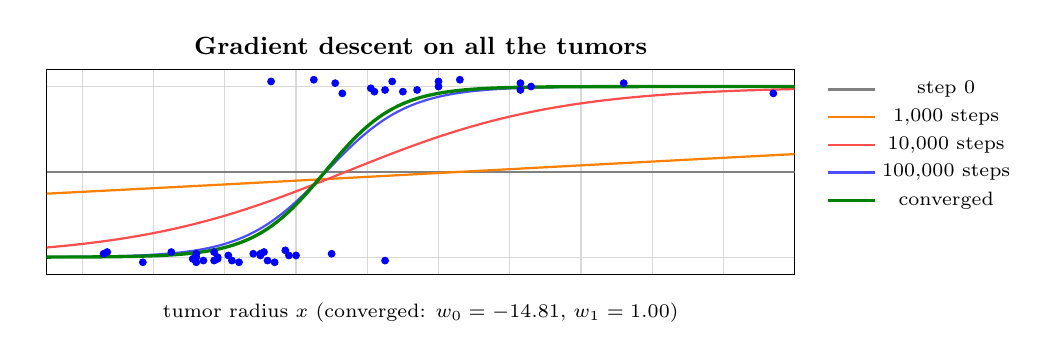
\begin{tikzpicture}
\begin{axis}[scale only axis, width=9.5cm, height=2.6cm,
    xmin=7, xmax=28, ymin=-0.1, ymax=1.1, enlargelimits=false,
    grid=major, grid style={gray!30}, major tick length=0pt,
    xticklabels={}, yticklabels={},
    title={\small\textbf{Gradient descent on all the tumors}}, title style={yshift=-4pt},
    xlabel={\scriptsize tumor radius $x$ (converged: $w_0 = -14.81$, $w_1 = 1.00$)}, label style={font=\scriptsize},
    legend pos=outer north east, legend style={font=\scriptsize, draw=none}]
\addplot[only marks, mark=*, blue, mark size=1.2pt, forget plot] coordinates {
  (8.6,0.02) (8.7,0.03) (9.7,-0.03) (10.5,0.03) (11.1,-0.01) (11.2,-0.00) (11.2,-0.03) (11.2,0.02)
  (11.4,-0.02) (11.7,0.03) (11.7,-0.02) (11.8,0.00) (11.8,-0.01) (12.1,0.01) (12.2,-0.02) (12.4,-0.03)
  (12.8,0.02) (13.0,0.02) (13.0,0.01) (13.1,0.03) (13.2,-0.02) (13.3,1.03) (13.4,-0.03) (13.7,0.04)
  (13.8,0.01) (14.0,0.01) (14.5,1.04) (15.0,0.02) (15.1,1.02) (15.3,0.96) (16.1,0.99) (16.2,0.97)
  (16.5,-0.02) (16.5,0.98) (16.7,1.03) (17.0,0.97) (17.4,0.98) (18.0,1.00) (18.0,1.03) (18.6,1.04)
  (20.3,1.02) (20.3,0.98) (20.6,1.00) (23.2,1.02) (27.4,0.96)};
\addplot[thick, gray, domain=7:28, samples=2] {0.5};
\addlegendentry{step 0}
\addplot[thick, orange, domain=7:28, samples=100] {1/(1+exp(-(-0.837+0.045*x)))};
\addlegendentry{1,000 steps}
\addplot[thick, red!70, domain=7:28, samples=100] {1/(1+exp(-(-5.156+0.335*x)))};
\addlegendentry{10,000 steps}
\addplot[thick, blue!70, domain=7:28, samples=150] {1/(1+exp(-(-12.925+0.871*x)))};
\addlegendentry{100,000 steps}
\addplot[very thick, green!50!black, domain=7:28, samples=150] {1/(1+exp(-(-14.81+x)))};
\addlegendentry{converged}
\end{axis}
\end{tikzpicture}
\par}
\end{keeptogether}

\begin{itemize}
  \item \textbf{Big idea:} identical to linear regression's update, except the prediction is $\sigma(\mathbf{w}^\top\mathbf{x}_n)$ instead of $\mathbf{w}^\top\mathbf{x}_n$.
  \item \textbf{No normal equation:} setting the derivative to 0 leaves $\mathbf{w}$ stuck inside $\sigma$, so gradient descent is the only way.
  \item SGD and mini-batch work the same as before. Standardizing the radius first makes it converge much faster.
\end{itemize}
\subsection*{Making Predictions}
\begin{keeptogether}
Plug a new tumor into the trained model ($w_0 = -14.81$, $w_1 = 1.00$) and predict cancer if $P \ge T$, where $T$ is a \textbf{threshold} you choose ($0.5$ by default). The boundary is the radius where the curve crosses $T$. With more features it's always a straight line or flat plane ($\mathbf{w}^\top\mathbf{x} = $ const): logistic regression is a \textbf{linear} classifier.

{\centering
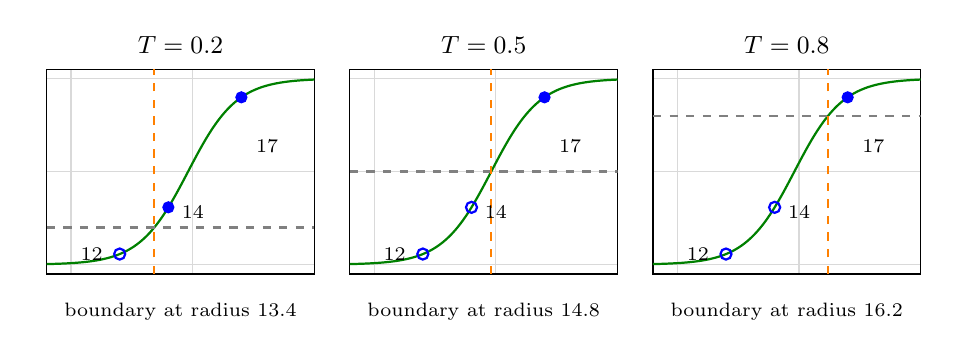
\begin{tikzpicture}
\begin{axis}[name=t2, scale only axis, width=3.4cm, height=2.6cm,
    xmin=9, xmax=20, ymin=-0.05, ymax=1.05, enlargelimits=false,
    grid=major, grid style={gray!30}, major tick length=0pt,
    xticklabels={}, yticklabels={},
    title={\small\textbf{$T = 0.2$}}, title style={yshift=-4pt},
    xlabel={\scriptsize boundary at radius 13.4}, label style={font=\scriptsize}]
\addplot[thick, green!50!black, domain=9:20, samples=120] {1/(1+exp(-(x-14.81)))};
\addplot[gray, dashed, thick] coordinates {(9,0.2) (20,0.2)};
\addplot[orange, dashed, thick] coordinates {(13.4,-0.05) (13.4,1.05)};
\addplot[only marks, mark=*, blue, mark size=2pt] coordinates {(14,0.308) (17,0.899)};
\addplot[only marks, mark=o, blue, mark size=2pt, thick] coordinates {(12,0.057)};
\node[font=\scriptsize, anchor=east] at (axis cs:11.7,0.057) {12};
\node[font=\scriptsize, anchor=west] at (axis cs:14.15,0.28) {14};
\node[font=\scriptsize, anchor=north west] at (axis cs:17.2,0.72) {17};
\end{axis}
\begin{axis}[name=t5, at={(t2.east)}, anchor=west, xshift=0.45cm,
    scale only axis, width=3.4cm, height=2.6cm,
    xmin=9, xmax=20, ymin=-0.05, ymax=1.05, enlargelimits=false,
    grid=major, grid style={gray!30}, major tick length=0pt,
    xticklabels={}, yticklabels={},
    title={\small\textbf{$T = 0.5$}}, title style={yshift=-4pt},
    xlabel={\scriptsize boundary at radius 14.8}, label style={font=\scriptsize}]
\addplot[thick, green!50!black, domain=9:20, samples=120] {1/(1+exp(-(x-14.81)))};
\addplot[gray, dashed, thick] coordinates {(9,0.5) (20,0.5)};
\addplot[orange, dashed, thick] coordinates {(14.8,-0.05) (14.8,1.05)};
\addplot[only marks, mark=*, blue, mark size=2pt] coordinates {(17,0.899)};
\addplot[only marks, mark=o, blue, mark size=2pt, thick] coordinates {(12,0.057) (14,0.308)};
\node[font=\scriptsize, anchor=east] at (axis cs:11.7,0.057) {12};
\node[font=\scriptsize, anchor=west] at (axis cs:14.15,0.28) {14};
\node[font=\scriptsize, anchor=north west] at (axis cs:17.2,0.72) {17};
\end{axis}
\begin{axis}[name=t8, at={(t5.east)}, anchor=west, xshift=0.45cm,
    scale only axis, width=3.4cm, height=2.6cm,
    xmin=9, xmax=20, ymin=-0.05, ymax=1.05, enlargelimits=false,
    grid=major, grid style={gray!30}, major tick length=0pt,
    xticklabels={}, yticklabels={},
    title={\small\textbf{$T = 0.8$}}, title style={yshift=-4pt},
    xlabel={\scriptsize boundary at radius 16.2}, label style={font=\scriptsize}]
\addplot[thick, green!50!black, domain=9:20, samples=120] {1/(1+exp(-(x-14.81)))};
\addplot[gray, dashed, thick] coordinates {(9,0.8) (20,0.8)};
\addplot[orange, dashed, thick] coordinates {(16.2,-0.05) (16.2,1.05)};
\addplot[only marks, mark=*, blue, mark size=2pt] coordinates {(17,0.899)};
\addplot[only marks, mark=o, blue, mark size=2pt, thick] coordinates {(12,0.057) (14,0.308)};
\node[font=\scriptsize, anchor=east] at (axis cs:11.7,0.057) {12};
\node[font=\scriptsize, anchor=west] at (axis cs:14.15,0.28) {14};
\node[font=\scriptsize, anchor=north west] at (axis cs:17.2,0.72) {17};
\end{axis}
\end{tikzpicture}
\par}
{\centering\scriptsize Tumors with radius 12, 14, 17 ($P = 0.06,\ 0.31,\ 0.90$). Filled: predict cancer. Hollow: predict not cancer.\par}
\end{keeptogether}

A tumor left of the boundary ($P < T$) is predicted not cancer ($t = 0$); right of it ($P \ge T$) is predicted cancer ($t = 1$). Raising $T$ moves the boundary right, so radius 14 goes from cancer at $T = 0.2$ to not cancer at $T = 0.5$.
\subsection*{Separable Data and Regularization}
\begin{keeptogether}
If one radius cleanly splits the classes, a steeper S always lowers the cross-entropy, so gradient descent pushes $w_1 \to \infty$ and the curve becomes a step: 100\% sure about everything. Fix: add a penalty on big weights,
\[
E(\mathbf{w}) + \frac{\lambda}{2}\|\mathbf{w}\|^2,
\]
so the weights stop at a finite value.

{\centering
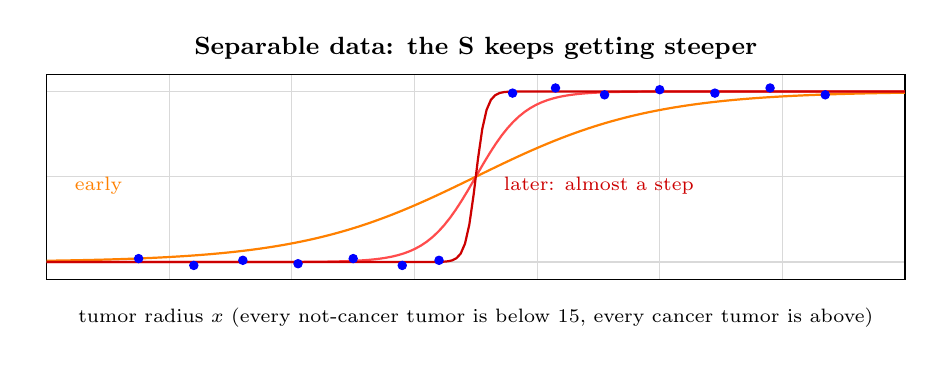
\begin{tikzpicture}
\begin{axis}[scale only axis, width=10.9cm, height=2.6cm,
    xmin=8, xmax=22, ymin=-0.1, ymax=1.1, enlargelimits=false,
    grid=major, grid style={gray!30}, major tick length=0pt,
    xticklabels={}, yticklabels={},
    title={\small\textbf{Separable data: the S keeps getting steeper}}, title style={yshift=-4pt},
    xlabel={\scriptsize tumor radius $x$ (every not-cancer tumor is below 15, every cancer tumor is above)}, label style={font=\scriptsize}]
\addplot[only marks, mark=*, blue, mark size=1.5pt] coordinates {
  (9.5,0.02) (10.4,-0.02) (11.2,0.01) (12.1,-0.01) (13.0,0.02) (13.8,-0.02) (14.4,0.01)
  (15.6,0.99) (16.3,1.02) (17.1,0.98) (18.0,1.01) (18.9,0.99) (19.8,1.02) (20.7,0.98)};
\addplot[thick, orange, domain=8:22, samples=150] {1/(1+exp(-0.7*(x-15)))};
\addplot[thick, red!70, domain=8:22, samples=150] {1/(1+exp(-2.5*(x-15)))};
\addplot[thick, red!80!black, domain=8:22, samples=200] {1/(1+exp(-12*(x-15)))};
\node[font=\scriptsize, orange, anchor=west] at (axis cs:8.3,0.45) {early};
\node[font=\scriptsize, red!80!black, anchor=west] at (axis cs:15.3,0.45) {later: almost a step};
\end{axis}
\end{tikzpicture}
\par}
\end{keeptogether}
